\index{类型!族的|(}%
\index{transport|(defstyle}%
因为在类型伦中\emph{依值类型}函数是必须的, 所以也需要一个依值类型版的\cref{lem:map}.
然而这并不容易获得, 因为如果 $f:\prd{x:A} B(x)$ 和 $p:x=y$, 那么 $f(x):B(x)$ 和 $f(y):B(y)$ 是不同类型的元素, \emph{事实上}, 甚至不能询问它们是否相等.
缺失的成分是, $p$ 本身给了一个关联 $B(x)$ 和 $B(y)$ 的方式.

它就是 \autoref{sec:identity-types} 中的``恒等的不可区分性''.
\index{恒等的不可区分性}%
现在介绍它的一个不同的名字和符号, 并开始使用.

\begin{lem}[Transport]
    \label{lem:transport}
    提供 $A$ 上的类型族 $P$ 和 $p:\id[A]xy$.
    则有一个函数 $\transf{p}:P(x)\to P(y)$.
\end{lem}

\begin{proof}[第一个证明]
    令$D:\prd{x,y:A} (\id{x}{y}) \to \type$ 为一个类型族, 其定义为
    \[D(x,y,p)\defeq P(x)\to P(y).\]
    那么有函数
    \begin{equation*}
        d\defeq\lam{x} \idfunc[P(x)]:\prd{x:A} D(x,x,\refl{x}),
    \end{equation*}
    于是归纳原理给出对于 $p:x= y$ 有 $\indid{A}(D,d,x,y,p):P(x)\to P(y)$, 也就是 $\transf p$ 的定义.
\end{proof}

\begin{proof}[第二个证明]
    通过归纳, 足以认为 $p$ 是 $\refl x$.
    在这个情况下, 可以令 $\transf{(\refl x)}:P(x)\to P(x)$ 为恒等函数.
\end{proof}

有时, 在 transport 符号上, 有必要把类型族 $P$ 用符号表示. 这种情况下, 可以写作 \[\transfib P p \blank : P(x) \to P(y).\]

回顾 $A$ 上的类型族 $P$ 可以被视作 $A$ 的元素的性质, 当 $x$ 是 $A$ 的元素且 $P(x)$ 有居留元时, 这个性质成立.
然后 transport 引理表示 $P$ 的平等性, 从在种意义上, 如果 $x$ 等于 $y$, 那么当且仅当 $P(y)$ 成立时 $P(x)$ 成立.
实际上, 以后可以看到如果 $x=y$ 则实际上 $P(x)$ 和 $P(y)$ 是\emph{等价的}.

拓扑学上, transportation 引理可以被视为纤维化上的``路径提升''操作.
\index{纤维化}%
\indexdef{全!空间}%
类型族 $P:A\to \type$ 被认为是基础空间 $A$ 上的\emph{纤维化}, 其中 $P(x)$ 是 $x$ 上的纤维, $\sm{x:A}P(x)$ 是纤维化的\define{全空间}, 其中第一投影 $\sm{x:A}P(x)\to A$.
纤维化的定义的性质是给定基础空间 $A$ 的一个路径 $p:x=y$, 和经过 $x$ 的纤维上的一个点 $u:P(x)$, 可以提升路径 $p$ 到全空间, 起点为 $u$ (而这个提升可以是连续完成的).
点 $\trans p u$ 可以被认为是这个被提升的路径的其他端点.
在类型论中, 也可以定义这个类型本身:

\begin{lem}[路径提升性质]
    \label{thm:path-lifting}
    \indexdef{路径!提升}%
    \indexdef{提升!路径}%
    令 $P:A\to\type$ 为一个经过 $A$ 的类型族, 并假设对于一些 $x:A$ 有 $u:P(x)$.
    然后对于任何 $p:x=y$, 有
    \begin{equation*}
        \mathsf{lift}(u,p):(x,u)=(y,\trans{p}{u})
    \end{equation*}
    在 $\sm{x:A}P(x)$, 于是 $\ap{\proj1}{\mathsf{lift}(u,p)} = p$.
\end{lem}
\begin{proof}
    留给读者.
    在\cref{sec:compute-sigma}会证明更通用的定理.
\end{proof}

在经典同伦论中, 纤维化被定义为\emph{存在}路径的提升的映射;
相比之下, 刚刚表明了, 在类型论中, 每个类型族都是一个\emph{指定的}``路径提升函数''.
这符合构造主义数学的哲学, 只有展示它, 才能说某个事物存在.
\index{类型伦中函数的连续性@类型伦中函数的``连续性''}%
它确保了路径提升具备良好的``连续性'', 因为类型伦中所有函数都是``连续的''.

\begin{rmk}
    尽管类型族 $P:A\to \type$ 被认为是像纤维化一样, 但广泛地说``纤维化 $P:A\to\type$'' 并不是一个好主意, 为这听起来像是在说基于底 $\type$ 和全空间 $A$ 的纤维结构.
    重复一遍, 当一个类型族 $P:A\to \type$ 被视为一个纤维化时, 它的底是 $A$ 而全空间是 $\sm{x:A} P(x)$.

    在讨论类型族时, 偶尔会使用其它拓扑术语.
    例如, 可能会把依赖函数 $f:\prd{x:A} P(x)$ 称作纤维化 $P$ 的\define{截面}
    \indexdef{截面!类型族的}%
    , 并说如果一个事物出现在所有 $P(x)$ 上, 那么说它是以\define{纤维方式}出现的.
    \indexdef{纤维方式}%

    例如, 一个截面 $f:\prd{x:A} P(x)$ 展示了 $P$ 是 ``纤维方式居留''.
\end{rmk}

\index{函数!依赖|(}
现在可以证明依赖版本的\cref{lem:map}.
拓扑上的直觉是, 给定 $f:\prd{x:A} P(x)$ 和路径 $p:\id[A]xy$, 可以应用 $f$ 到 $p$ 然后得到一条路径, 它在 $P$ 的全空间上, 并 ``lies over'' $p$, 如下图所示.

\begin{center}
    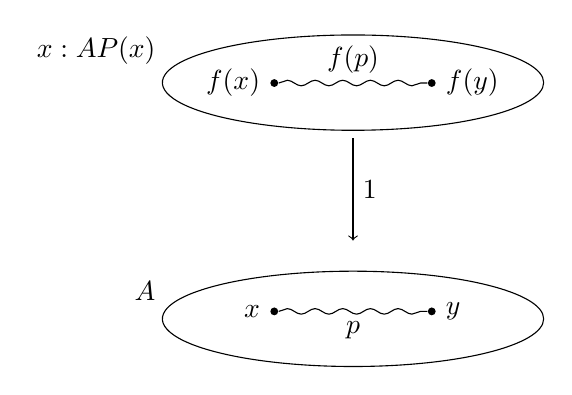
\begin{tikzpicture}[yscale=.5,xscale=2]
        \draw (0,0) arc (-90:170:8ex) node[anchor=south east] {$A$} arc (170:270:8ex);
        \draw (0,6) arc (-90:170:8ex) node[anchor=south east] {$\sm{x:A} P(x)$} arc (170:270:8ex);
        \draw[->] (0,5.8) -- node[auto] {$\proj1$} (0,3.2);
        \node[circle,fill,inner sep=1pt,label=left:{$x$}] (b1) at (-.5,1.4) {};
        \node[circle,fill,inner sep=1pt,label=right:{$y$}] (b2) at (.5,1.4) {};
        \draw[decorate,decoration={snake,amplitude=1}] (b1) -- node[auto,swap] {$p$} (b2);
        \node[circle,fill,inner sep=1pt,label=left:{$f(x)$}] (b1) at (-.5,7.2) {};
        \node[circle,fill,inner sep=1pt,label=right:{$f(y)$}] (b2) at (.5,7.2) {};
        \draw[decorate,decoration={snake,amplitude=1}] (b1) -- node[auto] {$f(p)$} (b2);
    \end{tikzpicture}
\end{center}

We \emph{can} obtain such a thing from \cref{lem:map}.
Given $f:\prd{x:A} P(x)$, we can define a non-dependent function $f':A\to \sm{x:A} P(x)$ by setting $f'(x)\defeq (x,f(x))$, and then consider $\ap{f'}{p} : f'(x) = f'(y)$.
Since $\proj1 \circ f' \jdeq \idfunc[A]$, by \cref{lem:ap-functor} we have $\ap{\proj1}{\ap{f'}{p}} = p$; thus $\ap{f'}{p}$ does ``lie over'' $p$ in this sense.
However, it is not obvious from the \emph{type} of $\ap{f'}{p}$ that it lies over any specific path in $A$ (in this case, $p$), which is sometimes important.

The solution is to use the transport lemma.
By \cref{thm:path-lifting} we have a canonical path $\mathsf{lift}(u,p)$ from $(x,u)$ to $(y,\trans p u)$ which lies over $p$.
Thus, any path from $u:P(x)$ to $v:P(y)$ lying over $p$ should factor through $\mathsf{lift}(u,p)$, essentially uniquely, by a path from $\trans p u$ to $v$ lying entirely in the fiber $P(y)$.
Thus, up to equivalence, it makes sense to define ``a path from $u$ to $v$ lying over $p:x=y$'' to mean a path $\trans p u = v$ in $P(y)$.
And, indeed, we can show that dependent functions produce such paths.

\begin{lem}[依值映射]
    \label{lem:mapdep}
    \indexdef{应用!依值函数到一个路径}%
    \indexdef{路径!依值函数的应用}%
    \indexdef{函数!依值!应用到路径}%
    \indexdef{动作!路径的依值函数的}%
    提供 $f:\prd{x: A} P(x)$; 然后有一个映射
    \[\apdfunc f : \prd{p:x=y}\big(\id[P(y)]{\trans p{f(x)}}{f(y)}\big).\]
\end{lem}

\begin{proof}[第一个证明]
    令 $D:\prd{x,y:A} (\id{x}{y}) \to \type$ 为一个如下定义的类型族
    \begin{equation*}
        D(x,y,p)\defeq \trans p {f(x)}= f(y).
    \end{equation*}
    然后 $D(x,x,\refl{x})$ 是 $\trans{(\refl{x})}{f(x)}= f(x)$.
    但是因为 $\trans{(\refl{x})}{f(x)}\jdeq f(x)$, 得到 $D(x,x,\refl{x})\jdeq (f(x)= f(x))$.
    因此, 有这个函数
    \begin{equation*}
        d\defeq\lam{x} \refl{f(x)}:\prd{x:A} D(x,x,\refl{x})
    \end{equation*}
    现在路径归纳给出对于每个 $p:x= y$ 有 $\apdfunc f(p):\trans p{f(x)}= f(y)$ .
\end{proof}

\begin{proof}[第二个证明]
    通过归纳, 可以假设 $p$ 是 $\refl x$.
    这个情况下, 所需的等式 $\trans{(\refl{x})}{f(x)}= f(x)$ 命题上成立.
\end{proof}

We will refer generally to paths which ``lie over other paths'' in this sense as \emph{dependent paths}.
\indexsee{dependent!path}{path, dependent}%
\index{path!dependent}%
They will play an increasingly important role starting in \cref{cha:hits}.
In \cref{sec:computational} we will see that for a few particular kinds of type families, there are equivalent ways to represent the notion of dependent paths that are sometimes more convenient.

现在回顾\cref{sec:pi-types}, 非依值类型函数 $f:A\to B$ 是依值函数 $f:\prd{x:A} P(x)$ 在 $P$ 是静态类型族 $P(x) \defeq B$ 的特殊情况.
这种情况下, $\apdfunc{f}$ 和 $\apfunc{f}$ 是密切相关的, 因为如下引理:

\begin{lem}
    \label{thm:trans-trivial}
    如果 $P:A\to\type$ 定义为 $P(x) \defeq B$ 对于固定的 $B:\type$, 那么对于任何 $x,y:A$ 和 $p:x=y$ 和 $b:B$ 有路径
    \[ \transconst Bpb : \transfib P p b = b. \]
\end{lem}
\begin{proof}[第一个证明]
    固定 $b:B$, 然后令 $D:\prd{x,y:A} (\id{x}{y}) \to \type$ 为一个类型族, 定义为
    \[ D(x,y,p) \defeq (\transfib P p b = b). \]
    然后 $D(x,x,\refl x)$ is $(\transfib P{\refl{x}}{b} = b)$, 通过 transporting 的计算规则与 $(b=b)$ 判断等同.
    因此, 有这个函数
    \[ d \defeq \lam{x} \refl{b} : \prd{x:A} D(x,x,\refl x). \]
    现在路径归纳可以给出所需的元素
    \narrowequation{
        \prd{x,y:A}{p:x=y}(\transfib P p b = b).}
\end{proof}
\begin{proof}[第二个证明]
    通过归纳, 可以假设 $y$ 是 $x$ 而且 $p$ 是 $\refl x$.
    但是 $\transfib P {\refl x} b \jdeq b$, 所以这种情况下必须证明 $b=b$, 为此可以使用 $\refl{b}$.
\end{proof}

因此, 对于任何 $x,y:A$ 和 $p:x=y$ 和 $f:A\to B$, 通过分别连接 $\transconst Bp{f(x)}$ 和它的反转, 得到函数
\begin{align}
    \big(f(x) = f(y)\big) &\to \big(\trans{p}{f(x)} = f(y)\big)\label{eq:ap-to-apd}
    \qquad\text{和} \\
    \big(\trans{p}{f(x)} = f(y)\big) &\to \big(f(x) = f(y)\big).\label{eq:apd-to-ap}
\end{align}
事实上, 这些函数反向等价(它的意义会在\cref{sec:basics-equivalences}引入), 并且它们关联了 $\apfunc f (p)$ 和 $\apdfunc f (p)$.

\begin{lem}
    \label{thm:apd-const}
    对于 $f:A\to B$ 和 $p:\id[A]xy$, 有
    \[ \apdfunc f(p) = \transconst B p{f(x)} \ct \apfunc f (p). \]
\end{lem}
\begin{proof}[第一个证明]
    令 $D:\prd{x,y:A} (\id xy) \to \type$ 为类型族, 定义为
    \[ D(x,y,p) \defeq \big(\apdfunc f (p) = \transconst Bp{f(x)} \ct \apfunc f (p)\big). \]
    因此有
    \[D(x,x,\refl x) \jdeq \big(\apdfunc f (\refl x) = \transconst B{\refl x}{f(x)} \ct \apfunc f ({\refl x})\big).\]
    通过定义, 这个类型中出现的三个路径都是 $\refl{f(x)}$, 所以有
    \[ \refl{\refl{f(x)}} : D(x,x,\refl x). \]
    于是, 路径归纳给出所需的元素 $\prd{x,y:A}{p:x=y} D(x,y,p)$.
\end{proof}
\begin{proof}[第二个证明]
    通过归纳, 足以假定 $y$ 是 $x$ 而且 $p$ 是 $\refl x$.
    这个情况下, 需要证明的是 $\refl{f(x)} = \refl{f(x)} \ct \refl{f(x)}$, 判断上为真.
\end{proof}

因为 $\apdfunc{f}$ 和 $\apfunc{f}$ 的类型不同, 使用不同的符号会更清晰.
% We may sometimes use a notation $\apd f p$ for $\apdfunc{f}(p)$, which is similar to the notation $\ap f p$ for $\apfunc{f}(p)$.

\index{函数!依值|)}%

至此, 希望读者开始找到一些通过恒等类型的归纳做证明的感觉.
从现在开始不再给出两种风格的证明, 而是使用更清晰和使用的 (大部分情况是更简明的第二种).
这里有一些实用的 transport 引理; 留给读者做证明 (用两种风格).

\begin{lem}
    \label{thm:transport-concat}
    给定 $P:A\to\type$ 和 $p:\id[A]xy$ 与 $q:\id[A]yz$ 并且 $u:P(x)$, 有
    \[ \trans{q}{\trans{p}{u}} = \trans{(p\ct q)}{u}. \]
\end{lem}

\begin{lem}
    \label{thm:transport-compose}
    对于函数 $f:A\to B$ 和类型族 $P:B\to\type$, 和任意 $p:\id[A]xy$ 与 $u:P(f(x))$, 有
    \[ \transfib{P\circ f}{p}{u} = \transfib{P}{\apfunc f(p)}{u}. \]
\end{lem}

\begin{lem}
    \label{thm:ap-transport}
    对于 $P,Q:A\to \type$ 和函数的族 $f:\prd{x:A} P(x)\to Q(x)$, 和任意 $p:\id[A]xy$ 与 $u:P(x)$, 有
    \[ \transfib{Q}{p}{f_x(u)} = f_y(\transfib{P}{p}{u}). \]
\end{lem}

\index{类型!族|)}%
\index{transport|)}